% Tabela comparando as máquinas
\begin{table}[htb]
	\newcommand \mesmo[1] {\multicolumn{2}{c}{#1}}
	\centering
	\caption{Características das máquinas utilizadas nos testes}%
	\label{tab:maquinas}
	%{
	\begin{tabular}{ccc}
		\toprule
		& Máquina A & Máquina B\\
		\midrule
		Sistema Operacional
			%& ---
			& \mesmo{\begin{tabular}{@{}c@{}}
				Windows 10 Home\\64 \textit{bits}\end{tabular}} \\
			%(10.0, Compilação 14393)
			%(10.0, Compilação 15063) \\
			%& ---
			%& 64 \textit{bits} \\
		\midrule
		\multirow{3}{*}{Processador}
			%& ---
			& \mesmo{Intel\textregistered\ Core\texttrademark} \\%, ~2.6GHz \\
			& i5 5200U
			& i7 6600U \\% CPU
			& 2.20 GHz
			& 2.50 GHz \\
			% Cores
			%& ---
			%& 2 \textit{cores}, 4 \textit{threads} \\
		\midrule
		\multirow{3}{*}{Memória Principal}
			% Tipo
			& DDR3
			& DDR4 \\
			% Tamanho
			& 6 GB
			& 8 GB \\
			% Frequência
			& 798.7 MHz
			& 1067 MHz \\
			%
			%& ---
			%&  \\
		\bottomrule
	\end{tabular}
\end{table}

\begin{table}[htb]
	\newcommand \mesmo[1] {\multicolumn{2}{c}{#1}}
	\centering
	\caption{\textit{Caches} das máquinas utilizadas nos testes}%
	\label{tab:caches}
	%{
	\begin{tabular}{ccc}
		\toprule
		\textit{Cache} & Máquina A & Máquina B\\
		\midrule
		L1
			& \mesmo{32 KB} \\
		L2
			& \mesmo{256 KB} \\
		L3
			& 3072 KB
			& 4096 KB \\
		\bottomrule
	\end{tabular}
\end{table}


%\begin{figure}
%	\centering
%	\caption{Saída do programa lstopo sobre as máquinas utilizadas}
%	\label{img:maquinas}
%	\begin{subfigure}{.4\textwidth}
%		\caption{Máquina A}
%		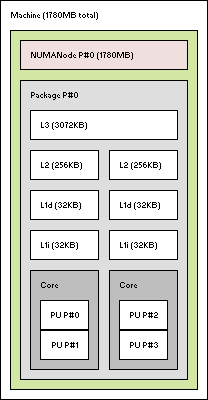
\includegraphics[width=\textwidth]{rec/img/MaqA}
%	\end{subfigure}
%	~
%	\begin{subfigure}{.4\textwidth}
%		\caption{Máquina B}
%		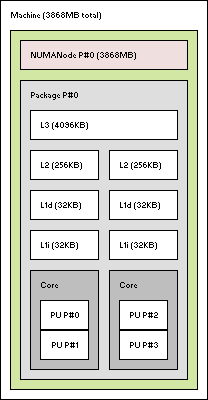
\includegraphics[width=\textwidth]{rec/img/MaqB}
%	\end{subfigure}
%
%\end{figure}